% !TeX root = RJwrapper.tex
\title{R Medicine 2020: The Power of Going Virtual}
\author{by Elizabeth J. Atkinson, Peter D. Higgins, Denise
Esserman, Michael J. Kane, Steven J. Schwager, Joseph B.
Rickert, Daniella Mark, Mara Alexeev, and Stephan Kadauke}

\maketitle

\abstract{%
The third annual R/Medicine conference was planned as a physical event
to be held in Philadelphia at the end of August 2020. However, a
nationwide lockdown induced by the COVID-19 pandemic required a swift
transition to a virtual conference. This article describes the
challenges and benefits we encountered with this transition and provides
an overview of the conference content.
}

\hypertarget{introduction}{%
\subsection{Introduction}\label{introduction}}

R/Medicine is an active working group of the R consortium, with the goal
of supporting R users in medicine, medical research, and related health
fields. The group includes a mix of statisticians and physicians who use
R regularly in their work, as well as members from RStudio and the R
Foundation.

The 2018 inaugural R/Medicine conference was a two day event held near
Yale University with Rob Tibshirani providing the initial keynote
address; each day began with a two hour tutorial. In 2019 the conference
was held in Boston and included, among others, keynote addresses by
Terry Therneau and Frank Harrell. Two half-day workshops were held on
the day prior to the conference.

In 2020, the R/Medicine Working Group organized the third annual
R/Medicine conference which was originally planned to be held in
Philadelphia. By early April 2020 it was clear that the conference would
need to be held virtually. This article describes some of the challenges
as well as unexpected benefits we encountered when pivoting to a virtual
conference, with the hope of providing useful information for other
conference organizers.

\hypertarget{conference-planning-and-logistics}{%
\subsection{Conference Planning and
Logistics}\label{conference-planning-and-logistics}}

Initial planning for the conference began in January 2020. By February,
we had identified keynote speakers and workshop leaders, and started
negotiations with a hotel near the Children's Hospital of Philadelphia
which was pegged as the site of the conference. However, by the
beginning of April we realized that we would need to switch to a virtual
event.

The initial challenge for the planning committee was identifying
technology that would allow us to run a main session of presentations,
teach short courses, and host Birds-of-a-Feather (BoF) activities that
allow like-minded R users to network and socialize. Because of our
limited budget we had limited choices for an online conferencing
platform. With help from the Linux Foundation, which provided
recommendations of some of the available conference platforms, we chose
to use Crowdcast (\url{https://www.crowdcast.io}). This tool was simple
to use for the attendees and the organizers, had a green room to line up
speakers, an interactive chat feature, and the ability to automatically
provide a recording of the session for replay immediately after its
conclusion. Compared to other conference platforms, Crowdcast has a
rather minimalist set of features. However, feedback from conference
participants confirmed that the user interface, consisting of a
single-track video feed and sidebar participant chat worked well. One
downside of Crowdcast was that it did not support screen readers or
closed captioning.

For the short courses we chose Zoom (\url{https://zoom.us}) as the
delivery platform, primarily because of its widespread use and because
of a mature breakout room functionality. We found that breakout rooms
are a useful tool for teaching, but should be used sparingly, because
the overhead of sending participants into breakout rooms can interrupt
the flow of teaching the material. For the \emph{Introduction to R for
Clinicians} course, we had a meet-and-greet breakout near the beginning
of the course as well as a final ``Hackathon'' breakout in which
participants were able to team up to design a dashboard.

Often, the most effective way to teach programming topics is live coding
\citep{Wilson2018}. Much effort has been devoted to create teaching
environments that allow participants to live code during a short course
without requiring installation of any software. In the R ecosystem, the
most notable and laudable effort in this regard is RStudio Cloud
(\url{https://rstudio.cloud}), which is based on the RStudio Server
Integrated Development Environment (IDE). From previous experience
teaching R to an audience of clinicians who have no programming
experience and are unfamiliar with the R ecosystem, we knew that the
RStudio Cloud environment could be challenging because it requires each
participant to first register a personal account on the platform before
being granted access to the training environment. To address this, we
created a training environment with pre-configured generic sequentially
numbered training accounts (e.g., \texttt{train001}, \texttt{train002},
etc.). After receiving training account credentials, a participant could
directly access their training environment from a web browser without
any further sign-ups. The training environment was implemented as a
Docker-based web application based on RStudio Server which was
configured with custom R packages and exercise files and hosted on a
cloud provider. The application is available for free online
\citep{arsptrain}.

Zoom was used for the BoF sessions, and we used Slack for back-channel
communication between the organizers, participants, and presenters. Some
Slack channels were created for participants while other channels were
limited to the conference planners. After the conclusion of the
conference, all the recorded presentations were loaded onto the
R/Medicine 2020 YouTube channel which is hosted by the R Consortium
-\citet{youtube1}. Since September 13, 2020 when the videos were
uploaded, there have been over 3,200 views. Registration and abstract
submission were facilitated by infrastructure provided by the Linux
Foundation. Google Sheets were used to centralize organization of the
program and the list of volunteers. We used Google Docs for creating
conference planning documents and Google Forms for course sign-ups and
surveys.

Since the \texttt{@r\_medicine} Twitter account has a large following
(2,557 as of June 2021), we used Twitter as the main outlet to promote
the event. We also directly engaged specific groups that we wanted to
participate to improve the conference experience, including R/Ladies,
Minorities in R, as well as medical professional organizations including
the American Association for Clinical Chemistry (AACC), and Mass
Spectrometry \& Advances in the Clinical Lab (MSACL).

\hypertarget{volunteers}{%
\subsubsection{Volunteers}\label{volunteers}}

The number of volunteers needed for the virtual conference was
significantly higher than for the previous in-person R/Medicine
conferences. For each short course we had at least one teaching
assistant for every 10 participants. Additionally, we had someone
monitoring the Zoom chat to escalate issues when necessary.

For the main session we had two moderators who alternated between
speakers in order to orient the upcoming speaker in the green room. We
also had a Crowdcast host who helped behind the scenes and moved
participants from one presentation to the next. One person was also in
charge of playing any of the talks that were pre-recorded. Each BoF room
had a facilitator. Because this was a virtual conference, we also
identified back-up volunteers in case there were power outages or issues
with internet access. Pre-conference training and discussion sessions
were held for short course teaching assistants. Pre-conference technical
checks were held prior to the conference for the speakers, instructors,
and volunteers.

\hypertarget{the-conference}{%
\subsection{The Conference}\label{the-conference}}

In the previous two years, attendance at each conference was around 150
participants. In 2020, 587 people registered for the conference,
including 225 students, 185 academics, 104 from industry, and 73 who
were working on COVID-19 related projects. Of these, 32\% were from
outside the United States coming from 43 countries (Figure
\ref{fig:map}). Of those who registered, 452 attended at least some
sessions live and 431 watched some sessions via the replay feature in
Crowdcast. The main conference was held over two days and included 4
keynote addresses, 16 regular talks, 11 lightning talks, and one panel
discussion. The schedule included three BoF time slots, each with 4-5
different topics.

\begin{Schunk}
\begin{figure}

{\centering 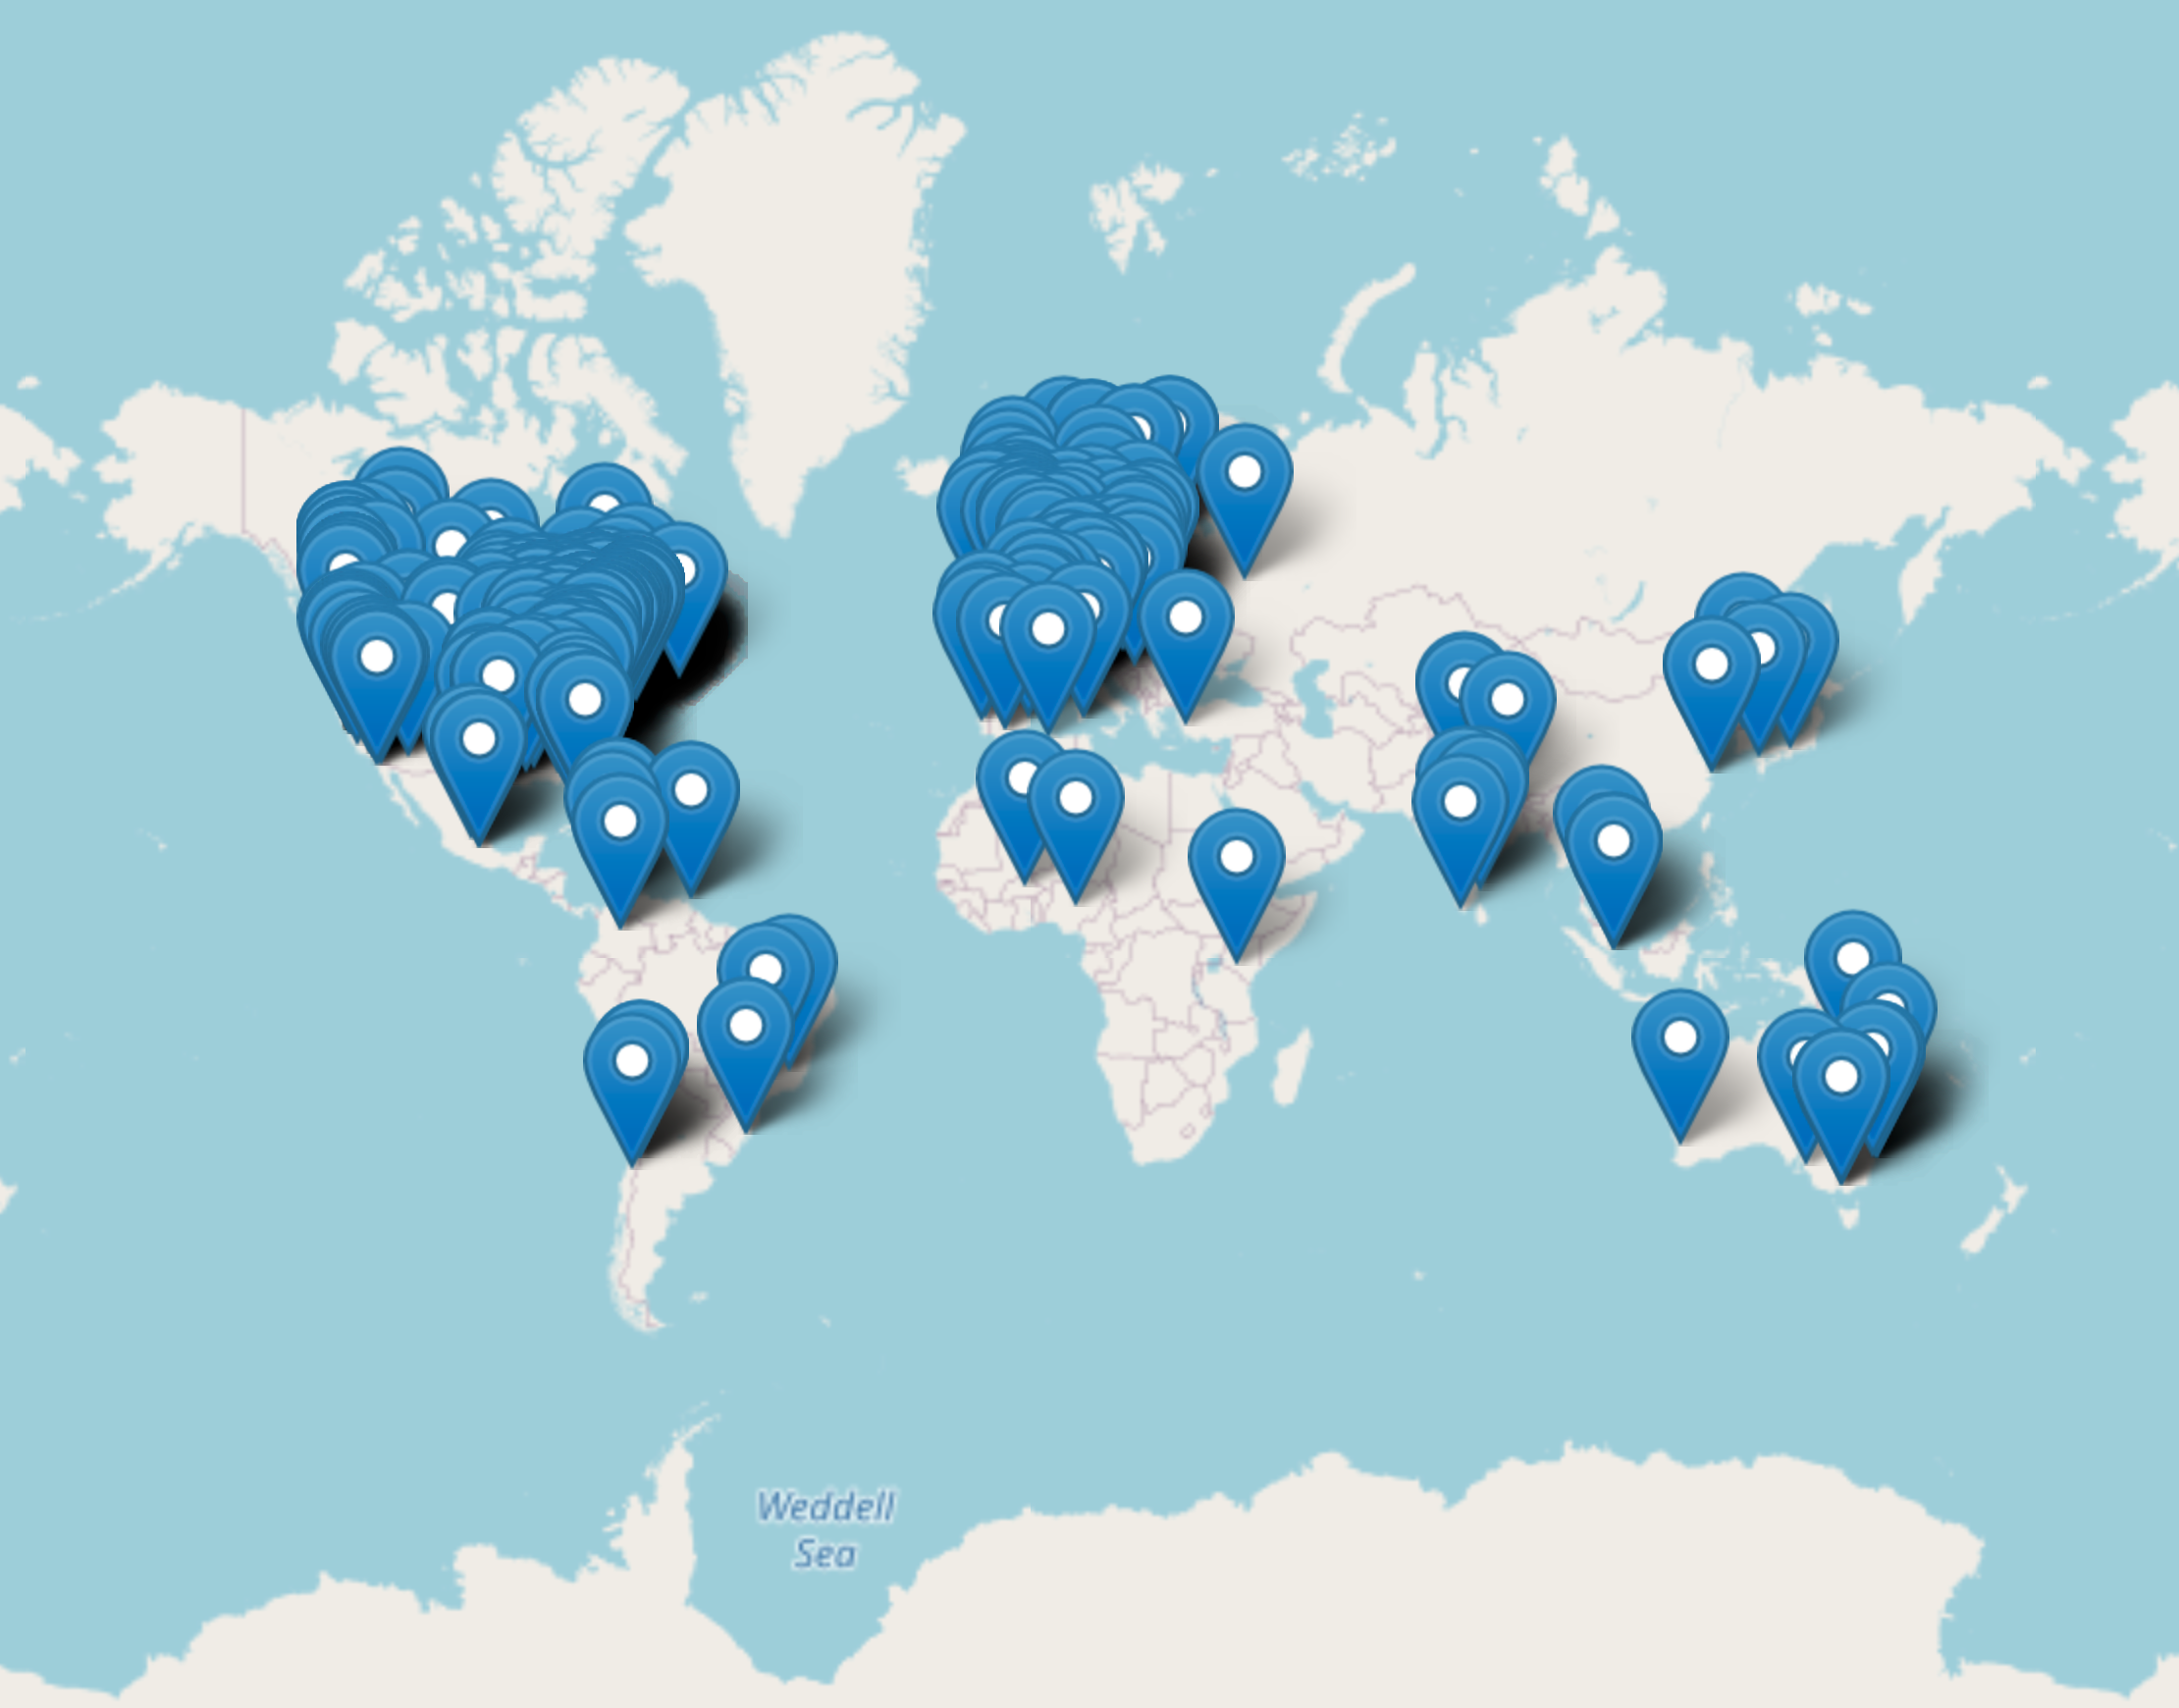
\includegraphics[width=0.7\linewidth]{Figure} 

}

\caption[Location of those who registered for the 2020 R/Medicine conference]{Location of those who registered for the 2020 R/Medicine conference}\label{fig:map}
\end{figure}
\end{Schunk}

We conducted a brief post-conference survey, which garnered 163
responses. We included the question ``How likely are you to recommend
this conference to a friend or colleague?'' with a 1-5 scale. The ``net
promoter score'', which was calculated by subtracting the fraction of
respondents rating the aforementioned question between 1-3 from the
fraction of respondents rating it a 5, was 55\%. Of all respondents,
98\% indicated that they planned to attend R/Medicine in the future.

\hypertarget{short-courses}{%
\subsubsection{Short Courses}\label{short-courses}}

Pre-conference events included two short courses presented on the day
prior to the conference. The first course, \emph{Introduction to R for
Clinicians}, is an adaptation of the popular \emph{Welcome to the
Tidyverse} course \citep{tidyclass} for an audience of healthcare
professionals and clinical researchers. The four-hour course placed
heavy emphasis on reproducibility and using R Markdown as a
computational document format and introduced fundamental concepts of
data visualization and data transformation using the \texttt{tidyverse}
set of tools \citep{Wickham2019}. Course materials \citep{introcourse}
and recordings \citep{introhear} are available online.

The second course, \emph{Introduction to Machine Learning with
Tidymodels}, was taught by Alison Hill and focused on the data
scientist/statistician audience. This four-hour course aimed to provide
a gentle introduction to machine learning with R using the modern suite
of predictive modeling packages called \texttt{tidymodels}. Participants
practiced building, evaluating, comparing, and tuning predictive models
interactively. The course introduced fundamental concepts including
resampling, overfitting, the holdout method, the bias-variance
trade-off, ensembling, cross-validation, and feature engineering; the
course materials \citep{tidycourse} is available online.

Attendance at the short courses was limited by request of the
instructors. The \emph{Introduction to R for Clinicians} class drew 143
participants, and 80 attended the \emph{Introduction to Machine Learning
with Tidymodels} course. Course recordings were available for anyone
registered for the conference.

\hypertarget{scientific-program}{%
\subsubsection{Scientific Program}\label{scientific-program}}

We received 43 abstracts and accepted 25. Additionally, we held space
for late-breaking COVID-19 related presentations and for two sponsors.
The Scientific Program of the conference was divided into six sessions,
each covering a broad theme.

\hypertarget{r-in-clinical-researchclinical-trials}{%
\paragraph{R in Clinical Research/Clinical
Trials:}\label{r-in-clinical-researchclinical-trials}}

This session started with a presentation by Daniela Witten, in which the
keynote speaker presented a theoretical framework for re-using data that
was collected for testing pre-specified hypotheses to drive new
hypothesis generation. Additional sessions focused on analyzing and
reporting clinical trial data as well as outlier and anomaly detection
in clinical trial data sets.

\hypertarget{collaborationreproducibility}{%
\paragraph{Collaboration/Reproducibility:}\label{collaborationreproducibility}}

The second session started with a keynote by Robert Gentleman in which
he outlined the value of large, well-curated data sets as well as how
the R ecosystem will be essential for developing new treatments as well
as validating and deploying healthcare analytics and clinical decision
support tools. Additional talks discussed the \texttt{\{drake\}} and
\texttt{\{holepunch\}} packages.

\hypertarget{new-analysis-approaches-and-packages}{%
\paragraph{New analysis approaches and
packages:}\label{new-analysis-approaches-and-packages}}

The last session of the first day started with a dazzling presentation
by Travis Gerke and Garrick Aden-Buie in which the speakers discussed
the development of internal R packages. An early prototype of a package
for creating CONSORT diagrams was presented, as well as summaries of
more mature packages including \texttt{\{gtsummary\}},
\texttt{\{nDSPA\}}, and \texttt{\{treeheatr\}}.

\hypertarget{r-in-clinical-practice-education-and-bioethics}{%
\paragraph{R in Clinical Practice, Education, and
Bioethics:}\label{r-in-clinical-practice-education-and-bioethics}}

The first session of the second conference day started with a keynote
speech by Ewen Harrison in which he highlighted the flexibility and ease
of using R which makes it an ideal platform for clinician-researchers or
other researchers who are not primarily programmers, as well as the
collaborative nature of the R community. Additional presentations
discussed the role of R in processing laboratory data in clinical
practice as well as teaching R to healthcare professionals. Finally, a
team presentation by Joy Payton and Paulette McRae highlighted the
problematic history of racism in medical research and practice,
discussed root causes of bias in data, and offered suggestions to
mitigate these biases.

\hypertarget{dashboards-and-shiny-apps}{%
\paragraph{Dashboards and Shiny Apps:}\label{dashboards-and-shiny-apps}}

This session discussed a variety of web applications developed using the
Shiny framework that were being used either in clinical practice or
clinical research.

\hypertarget{covid-19-research}{%
\paragraph{COVID-19 research:}\label{covid-19-research}}

The final session started with a keynote by Patrick Mathias, who shared
his experience directing both the clinical operations and operational
analytics efforts of one of the busiest clinical COVID-19 testing
laboratories in the United States \citep{covid}. Additional
presentations highlighted the role R has played in coordinating the
response to the COVID-19 pandemic.

\hypertarget{lessons-learned}{%
\subsection{Lessons learned}\label{lessons-learned}}

Overall, the conference succeeded well beyond our expectations. Some of
the lessons we learned are as follows.

\begin{itemize}
\item
  The chat feature helped build community and allowed active
  participation in the conference. For instance, some presenters
  tag-teamed where one person presented and another answered questions
  via chat as they arose. Other presenters had pre-recorded their talk
  and were thus able to answer live questions during the playback of
  their presentation.
\item
  Slack was essential for the behind-the-scenes coordination, especially
  as issues arose. Additionally, we had participants create their own
  channels and Zoom sessions for further discussion on certain topics.
\item
  Having back-ups for all the major coordinating roles was essential.
  Fortunately we had limited issues, but one keynote speaker experienced
  a power outage, leading to an unavoidable delay.
\item
  Although Crowdcast allows for smooth transitioning between speakers,
  time to transition between presenters needs to be built into the
  schedule, since presenters run over, technical issues emerge, and
  bio-breaks are important. It is also wise to build in some flex-time
  in case there are technical difficulties.
\item
  During the presentations it was challenging to let speakers know when
  they were running out of time. All moderators downloaded a app to
  their phones that allowed them to play a doorbell sound to indicate to
  the speaker that their time is almost up, however that was not always
  effective. For 2021 we are planning to require that lightning talks be
  pre-recorded.
\item
  Having a virtual meeting greatly expanded our reach. In 2019 we held
  the conference in Boston and had roughly 150 attendees from a handful
  of countries whereas in 2020 we had 452 attendees from 43 countries.
  We hope that the larger attendance will increase our impact as well as
  our ability to obtain sponsors for future conferences.
\item
  Recruitment for high caliber keynote speakers was perhaps easier
  because the time commitment and travel effort were substantially less
  than for an in-person conference.
\end{itemize}

\hypertarget{sponsors}{%
\subsection{Sponsors}\label{sponsors}}

We would like to thank all the sponsors that supported the 2020
conference: American Association for Clinical Chemistry (AACC),
Children's Hospital of Philadelphia (CHOP), Association for Mass
Spectrometry \& Advances in the Clinical Lab (MSACL), Procogia, the R
Consortium, RStudio, and Yale School of Public Health.

\hypertarget{acknowledgements}{%
\subsection{Acknowledgements}\label{acknowledgements}}

As members of the R/Medicine 2020 Organizing and Programming Committees,
we would like to thank all the volunteers who contributed to the success
of the conference, the course instructors and teaching assistants, the
keynote and contributed speakers, and all the attendees who dialed in
from around the globe.

\hypertarget{links}{%
\subsection{Links}\label{links}}

Further information about R/Medicine 2020 and the contributions
presented during the conference can be found at the conference website:
\url{https://events.linuxfoundation.org/r-medicine/}

\bibliography{Rmed2020-Rjournal.bib}

\address{%
Elizabeth J. Atkinson\\
Department of Quantitative Health Sciences, Mayo Clinic\\%
200 First Street SW\\ Rochester, MN 55905\\
%
%
\textit{ORCiD: \href{https://orcid.org/0000-0002-1191-3775}{0000-0002-1191-3775}}\\%
\href{mailto:atkinson@mayo.edu}{\nolinkurl{atkinson@mayo.edu}}%
}

\address{%
Peter D. Higgins\\
Department of Internal Medicine, University of Michigan Health\\%
1500 E Medical Center Dr.\\ Ann Arbor, MI 48109\\
%
%
%
\href{mailto:phiggins@med.umich.edu}{\nolinkurl{phiggins@med.umich.edu}}%
}

\address{%
Denise Esserman\\
Department of Biostatistics, Yale School of Public Health\\%
300 George Street, Ste 555\\ New Haven, CT 06511\\
%
%
%
\href{mailto:denise.esserman@yale.edu}{\nolinkurl{denise.esserman@yale.edu}}%
}

\address{%
Michael J. Kane\\
Department of Biostatistics, Yale School of Public Health\\%
300 George Street, Ste 555\\ New Haven, CT 06511\\
%
%
%
\href{mailto:michael.kane@yale.edu}{\nolinkurl{michael.kane@yale.edu}}%
}

\address{%
Steven J. Schwager\\
Cornell University\\%
129 Garden Ave.\\ Ithaca, NY 14853\\
%
%
%
\href{mailto:steven.schwager@cornell.edu}{\nolinkurl{steven.schwager@cornell.edu}}%
}

\address{%
Joseph B. Rickert\\
R Consortium, RStudio\\%
548 Market St.\\ San Francisco, CA 94104\\
%
%
%
\href{mailto:joseph.rickert@rstudio.edu}{\nolinkurl{joseph.rickert@rstudio.edu}}%
}

\address{%
Daniella Mark\\
Procogia\\%
3600 136th Pl SE Suite 300\\ Bellevue, WA 98006\\
%
%
%
\href{mailto:daniella@procogia.com}{\nolinkurl{daniella@procogia.com}}%
}

\address{%
Mara Alexeev\\
Department of Biomedical Informatics, Boston Children's Hospital\\%
10 Shattuck Street, Suite 514\\ Boston, MA 02115\\
%
%
%
\href{mailto:mara.alexeev@gmail.com}{\nolinkurl{mara.alexeev@gmail.com}}%
}

\address{%
Stephan Kadauke\\
Department of Pathology and Laboratory Medicine, Children's Hospital of
Philadelphia, Perelman School of Medicine, University of Pennsylvania\\%
3401 Civic Center Blvd.\\ Philadelphia, PA 19104\\
%
%
\textit{ORCiD: \href{https://orcid.org/0000-0003-2996-8034}{0000-0003-2996-8034}}\\%
\href{mailto:kadaukes@chop.edu}{\nolinkurl{kadaukes@chop.edu}}%
}
